\section[Using voters list to map population in the Sahel]{Data hybridization for population mapping in Niger}

% TODO reformuler pour avoir plus de
% Importance mapping populaton
% different interest evolutioj
% question of representation

% data source probleù
% indirect imputation
% mapping

Knowing where people live is essential to the design and the evaluation of policies or interventions targetting populations. Population maps is thus an important tool for policy makers, or for actors of social policy or relief actions. Meanwhile, in data poor settings, the quest for precise and exact mapping of population has long proved an illusory goal, for reasons that touch both on the paucity of data, and on technical mapping issues.

This  project is exploring an innovative approach to mapping of populations in resource-limited settings. Using voters registration lists, a data source seldom used in demography, we will endeavour to offer a map of population in Niger that will be easily callable and usable by different actors intervening in Niger. To do this, we will challenge current practice in population mapping, and will aim at producing a point map, more adapted to daily usage than raster surfaces.

In the rest of this documents, we will first take a quick historical detour to better understand how our work is justified by an under-investment in population data sources in former French colonies, and how it is also situated in a long standing tradition of population mapping methods. We will then present the data sources we are using, and will discuss the methods use. Finally, we will describe the outputs we hope to produce by the end of the quarter.


\subsection{Mapping populations in sub-Saharan : a historical challenge}

\subsubsection{Data issues}

The first population  map can be traced to Crome's 1785 \textit{Groessen-Karte von Europa} \cite{klawe_population_1973}, in the time at which Foucault dates the "discovery of population"\cite{foucault2004securite}, thus hinting to how the concept of a governed population is consusbstantial to the localization of this population. Meanwhile, the production of these maps necessitates the availability and the processing of amounts of data that grow exponentially with the desired level of details. In countries that were formerly colonized by the French powers, the investment necessary to produce this geolocalized data on population has seldom been done. In the first movements of colonization, maps were mainly produced by the military, and in 1902, Paul Pelet's very first \textit{Atlas des colonies française}\cite{pelet1902atlas} did not include a lot on
information outside of topographic data\cite{zimmermann_atlas_1903}. Additionally, there was a radical choice made to use spellings for places in colonies that were adapted to metropolitan French rather than to local languages\cite{zimmermann_atlas_1903} The second period of colonisation was more interested in economic and commercial exploitation, and thus, the 1922's \textit{Exposition Coloniale} showed some progress in the mapping of geologic and natural resources, but still no population mapping was produced\cite{rambert_cartographie_1922}. In 1929, a first map of the population density was produced for Sénégal, using indirect methods to estimate the size of communities, using the amount collected for personnal taxes by local authorities\cite{rousseau_population_1929}.
This undervaluation of human data was prolunged in the structures that were left after the decolonizations\cite{lohle1999etat}, and reinforced by structural underinvestment in statistical systems in sub-saharan Africa\cite{jerven2013poor}. As a result, the main source of data for population size estimation in most sub-Saharan countries are census, that are performed at best every ten years. In countries with dynamic demographies, this means that most population estimations used are either outdated, or heavily modelled for projection purposes. There is a blatant need to find new data sources to estimate the size of local communities, that are updated more frequently, and are valid at local level.


%% DATA HYBRIDATION

\subsubsection{Methodological questions}

Mapping populations is a tricky task. In contrast to geological data or natural features, population is non continuous in space, and is changing very quickly. In 1935, Fawcett discerned three facts one may want to describe in a population map\cite{fawcett1935population} :
\begin{enumerate}
	\item The actual number of the people within given areas
	\item The density of the population
	\item The grouping, or arrangement, of the population.
\end{enumerate}
Each of these facts require a different type of mapping. The number of people in an area can be communicated through discretization of space, and association of a number of inhabitants in each subzone. Density mapping necessitates a more continuous approach to mapping, in terms of scale and of color scale. Arrangement of population can be shown through the plotting of points representing settlements, and with size representing the number of inhabitants. Each of these require different amounts and nature of primary data, and different computational approaches.

The latest advances in population mapping are geared towards the production of density surfaces, presenting a continuous description of where populations live on a territory\cite{linard2012population}. This new approach is made possible by the availability of large aggregate datasets for land use, and other usable covariates\cite{linard2011assessing}, and the computational ability to interpolate these  different data sources for popualtion distribution\cite{stevens2015disaggregating}.

Meanwhile, this approach presents two main problems that make its result of little use in country like Niger. First, the output format if these maps, a raster of population distribution, is of little use at a local level, where actors typically use places name and not GPS coordinates. Second, in countries with little urbanization, and poor population data, these rasters end up displaying an overlay of covariate layers more than they present a credible distribution of populations.

Moreover, if this top-down approach is useful to provide macro-level perspectives on population distribution, it is not useful for local level use. Local actors typically think in terms of places names, more than in terms of GPS coordinates. Additionaly, attractivity of a urban center for rural population is hard to model through macro level covariates, as it often depends on such factors as tradition, habits or administrative border drawing, as is evident in Figure 1.

\begin{figure}
	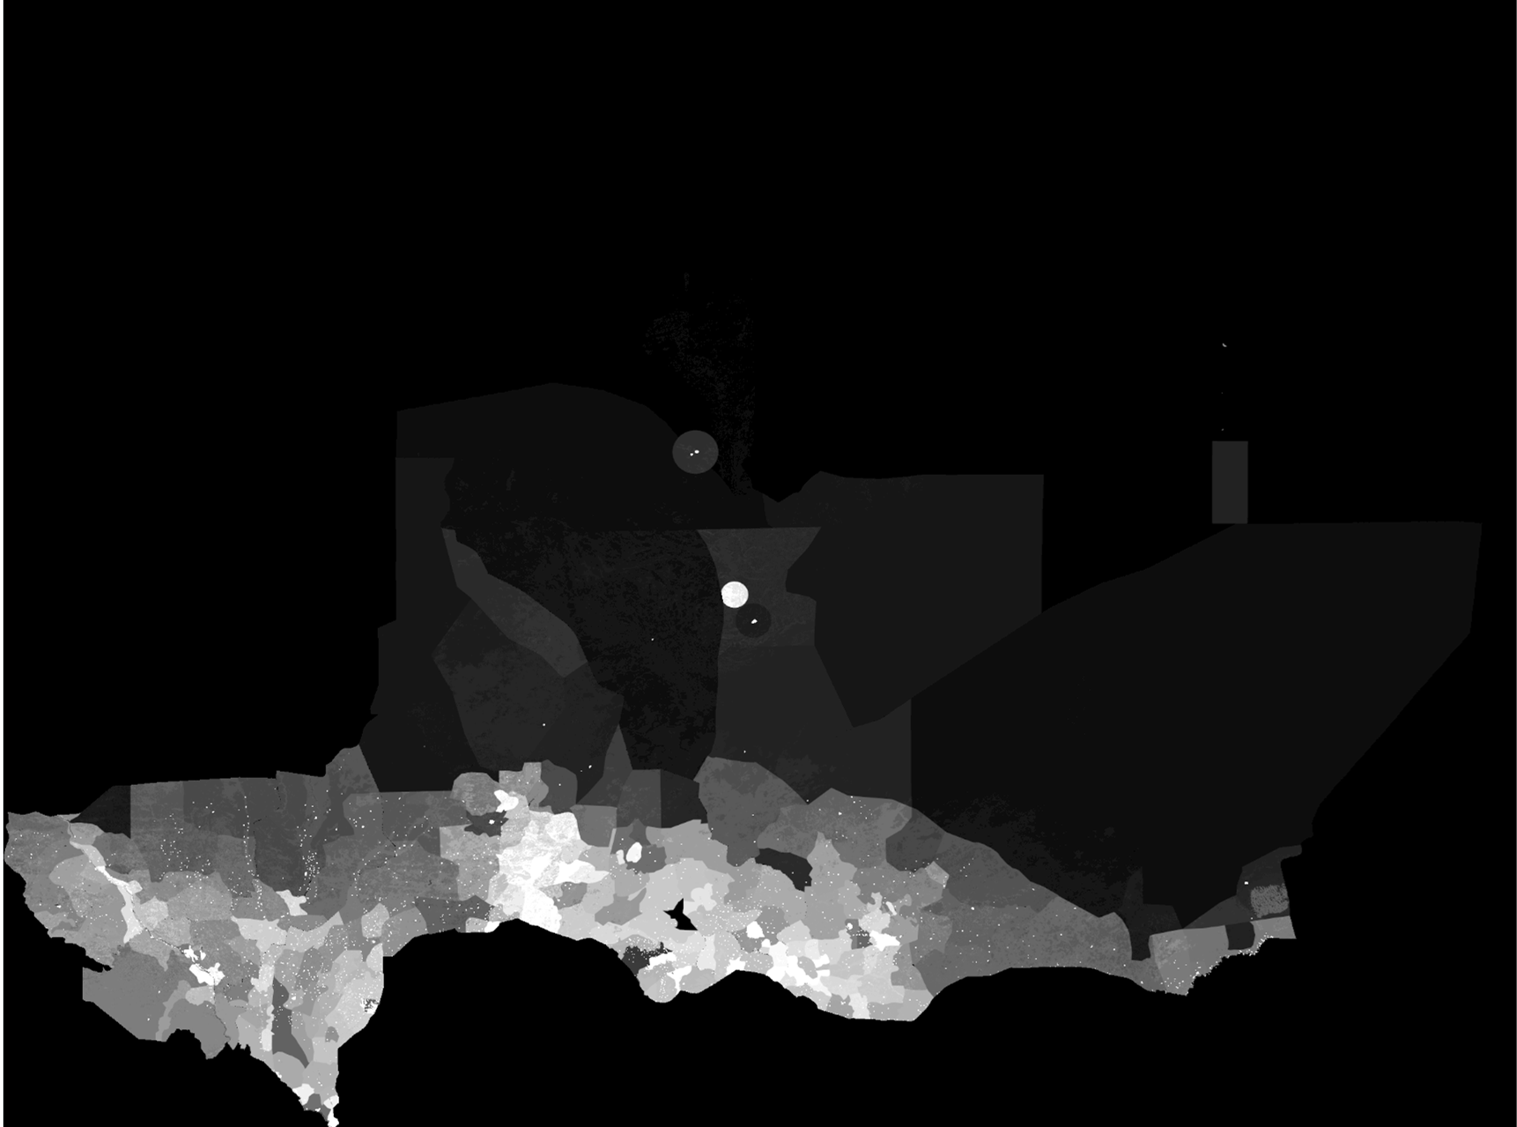
\includegraphics[width=15cm]{figure/WORLDPOP_Niger.png}
	\caption{Mapping of Niger population from AFRIPOP}
\end{figure}

In order to offer more useful maps for local actors, we will use an approach supported by very minimal modelling of primary population data distribution, and geared towards the anchoring of population in callable localisation names.

\subsection{Project concept}

\subsubsection{Data sources}

\paragraph{Voters list as a demographic Datasource} A data source that is, to our knowledge, seldom used to inform population mapping for public health purposes, is voters registration lists. There is meanwhile a case to be made for the use of voters' registration data to estimate size of populations. By definition, voters' registration should aim at being as complete as possible a register of adults in the nation. Moreover, in most democracies, some form of national elections are held at least  every five years, leading to an update at least partial of voters' registrations. In sub-Saharan Africa, between the years 2015 and 2016, 27 countries were supposed to hold national elections, leading to a theoretical registration of more than half of the adult population of the continent. Finally, for transparency and accountability reasons, electors registries are usually supposed to be easily accessible.

Due to the sensitive and political use of these data, the quality of voters registries are often described as not being trustworthy. On other hand, for the same sensitivity reasons, voters registries are receiving a very high level of scrutiny from many different actors, and are audited sometimes multiple times before validation. This level of scrutiny before validation is much higher than the attention given to a lot of studies or other often used data sources.

\paragraph{The Niger 2016 elections voters registry} In Niger, presidential and parlementary elections were held in February 2016. Voters lists were updated during the second half of the year 2015, under the supervision and control of a mission of the Office International de la Francophonie (OIF). The operations for registration of voters were conducted during the third quarter of 2015\footnote{http://www.ceni-niger.org/article-region/#more-24}. A first version of the voters list was published on December 21, 2015, tallying 7,569,172 voters, out of 8,569,309 that were expected based on the 2012 census\footnote{http://www.iinanews.org/page/public/news_details.aspx?id=98929&NL=True}

Final lists were validated in early January 2016 after being corrected for some incoherencies noted by the supervisory body\footnot{http://www.nigerinter.com/2016/01/le-fichier-electoral-du-niger-valable-sous-reserves/}. A final report on these lists was published in may 2016\footnote{http://www.nigerinter.com/2016/05/remise-officielle-du-rapport-du-fichier-electoral-au-ministre-detat-a-linterieur-par-le-cfeb/}. The Comission Electorale Nationale Independante (CENI) later made these lists fully available on its website, from which we extracted, anonymized and formatted the lists.

\paragraph{RENALOC and RENACOM} The \textit{Répertoire National des Localités} (RENALOC) is a geolocalized repertory of all localities in Niger.  The 2012 version was downloaded as a pdf file from the \textit{Institut National de la Statistique} (INS) website. The tables were extracted in bulk from this file using the Tabula Package, and then processed in Python to recompose the geographic structure of the document. The final data consists in 34507 localities, for which the INS provides the number of inhabitants, by gender, as well as the number of households, and the number of agricultural households. For most of the localities, a GPS coordinate is recorded, as well as the type of locality (neighborhood, village, camp, water well, hamlet).

The 2006 version, named RENACOM, was retrieved in tabular format directly from the INS website.

\paragraph{OpenStreetMap} Additional geolocalization method will be extracted from OpenStreetMap (OSM), using the python api for OSM.

\subsubsection{Objectives and Methods}

This project has three distinct but complementary objectives :
\begin{description}
	\item[Population estimation] We model Niger population, using the voters list by precinct as a primary covariate. Moreover, we model age structure of the population at local level using the age of registered voters. To do this, we combine traditionnal demography and Machine Learning (ML) methods, to get a proper estimation of uncertainty at locality level.
	\item[Name Matching] We already noted that different spelling of locality names are in use in Niger. We have no reason to privilegy on spelling over another for our project. Moreover, we want users of our map to be able to use whichever writing they prefer. Using our four data sources, we will offer a matching of different spellings of same names. This matching will be made using a combination of direct correction, unsupervised and supervised learning approaches. The output of this work will be, at the same time, a database, and a trained prediction algorithm able to offer a suitable guess to users using unknown spellings of localities.
	\item[Locality mapping] The three data sources for localization (RENALOC, RENACOM, OSM) have GPS coordinates for different subsets of localities in Niger, with some common coverage. It appears that RENALOC GPS coordinates are biased, and that OSM coordinates are sometimes rough estimates. We will try and correct GPS coordinates when needed, and map localities based on these coordinates.
\end{description}

Based on these objectives, the output of the project for the quarter will  be to produce a simple dashboard server, allowing a simple and usable display of our results. This dashboard will have the following feature :
\begin{enumerate}
	\item An interactive map of Niger localities, selectable by clicking, or panning for multiple selection
	\item An estimation of the population in the localities currently selected on the map
	\item An histogram representing the age structure of the population in the localities currently selected on the map
	\item A search box through which the user will be able to search for a given localiy. Unknown localities will return a list of probable similar places.
\end{enumerate}

Additional features of this dashboard may be, in no particular order : the display of uncertainty in population and age structure, the differentiation of recorded voters and extrapolated population, by age group, the ability to explore different modelling options.
